% Options for packages loaded elsewhere
\PassOptionsToPackage{unicode}{hyperref}
\PassOptionsToPackage{hyphens}{url}
\PassOptionsToPackage{dvipsnames,svgnames*,x11names*}{xcolor}
%
\documentclass[
]{article}
\usepackage{lmodern}
\usepackage{amssymb,amsmath}
\usepackage{ifxetex,ifluatex}
\ifnum 0\ifxetex 1\fi\ifluatex 1\fi=0 % if pdftex
  \usepackage[T1]{fontenc}
  \usepackage[utf8]{inputenc}
  \usepackage{textcomp} % provide euro and other symbols
\else % if luatex or xetex
  \usepackage{unicode-math}
  \defaultfontfeatures{Scale=MatchLowercase}
  \defaultfontfeatures[\rmfamily]{Ligatures=TeX,Scale=1}
\fi
% Use upquote if available, for straight quotes in verbatim environments
\IfFileExists{upquote.sty}{\usepackage{upquote}}{}
\IfFileExists{microtype.sty}{% use microtype if available
  \usepackage[]{microtype}
  \UseMicrotypeSet[protrusion]{basicmath} % disable protrusion for tt fonts
}{}
\makeatletter
\@ifundefined{KOMAClassName}{% if non-KOMA class
  \IfFileExists{parskip.sty}{%
    \usepackage{parskip}
  }{% else
    \setlength{\parindent}{0pt}
    \setlength{\parskip}{6pt plus 2pt minus 1pt}}
}{% if KOMA class
  \KOMAoptions{parskip=half}}
\makeatother
\usepackage{xcolor}
\IfFileExists{xurl.sty}{\usepackage{xurl}}{} % add URL line breaks if available
\IfFileExists{bookmark.sty}{\usepackage{bookmark}}{\usepackage{hyperref}}
\hypersetup{
  pdftitle={Homework 7},
  pdfauthor={Yunting Chiu},
  colorlinks=true,
  linkcolor=red,
  filecolor=Maroon,
  citecolor=Blue,
  urlcolor=blue,
  pdfcreator={LaTeX via pandoc}}
\urlstyle{same} % disable monospaced font for URLs
\usepackage[margin=1in]{geometry}
\usepackage{color}
\usepackage{fancyvrb}
\newcommand{\VerbBar}{|}
\newcommand{\VERB}{\Verb[commandchars=\\\{\}]}
\DefineVerbatimEnvironment{Highlighting}{Verbatim}{commandchars=\\\{\}}
% Add ',fontsize=\small' for more characters per line
\usepackage{framed}
\definecolor{shadecolor}{RGB}{248,248,248}
\newenvironment{Shaded}{\begin{snugshade}}{\end{snugshade}}
\newcommand{\AlertTok}[1]{\textcolor[rgb]{0.94,0.16,0.16}{#1}}
\newcommand{\AnnotationTok}[1]{\textcolor[rgb]{0.56,0.35,0.01}{\textbf{\textit{#1}}}}
\newcommand{\AttributeTok}[1]{\textcolor[rgb]{0.77,0.63,0.00}{#1}}
\newcommand{\BaseNTok}[1]{\textcolor[rgb]{0.00,0.00,0.81}{#1}}
\newcommand{\BuiltInTok}[1]{#1}
\newcommand{\CharTok}[1]{\textcolor[rgb]{0.31,0.60,0.02}{#1}}
\newcommand{\CommentTok}[1]{\textcolor[rgb]{0.56,0.35,0.01}{\textit{#1}}}
\newcommand{\CommentVarTok}[1]{\textcolor[rgb]{0.56,0.35,0.01}{\textbf{\textit{#1}}}}
\newcommand{\ConstantTok}[1]{\textcolor[rgb]{0.00,0.00,0.00}{#1}}
\newcommand{\ControlFlowTok}[1]{\textcolor[rgb]{0.13,0.29,0.53}{\textbf{#1}}}
\newcommand{\DataTypeTok}[1]{\textcolor[rgb]{0.13,0.29,0.53}{#1}}
\newcommand{\DecValTok}[1]{\textcolor[rgb]{0.00,0.00,0.81}{#1}}
\newcommand{\DocumentationTok}[1]{\textcolor[rgb]{0.56,0.35,0.01}{\textbf{\textit{#1}}}}
\newcommand{\ErrorTok}[1]{\textcolor[rgb]{0.64,0.00,0.00}{\textbf{#1}}}
\newcommand{\ExtensionTok}[1]{#1}
\newcommand{\FloatTok}[1]{\textcolor[rgb]{0.00,0.00,0.81}{#1}}
\newcommand{\FunctionTok}[1]{\textcolor[rgb]{0.00,0.00,0.00}{#1}}
\newcommand{\ImportTok}[1]{#1}
\newcommand{\InformationTok}[1]{\textcolor[rgb]{0.56,0.35,0.01}{\textbf{\textit{#1}}}}
\newcommand{\KeywordTok}[1]{\textcolor[rgb]{0.13,0.29,0.53}{\textbf{#1}}}
\newcommand{\NormalTok}[1]{#1}
\newcommand{\OperatorTok}[1]{\textcolor[rgb]{0.81,0.36,0.00}{\textbf{#1}}}
\newcommand{\OtherTok}[1]{\textcolor[rgb]{0.56,0.35,0.01}{#1}}
\newcommand{\PreprocessorTok}[1]{\textcolor[rgb]{0.56,0.35,0.01}{\textit{#1}}}
\newcommand{\RegionMarkerTok}[1]{#1}
\newcommand{\SpecialCharTok}[1]{\textcolor[rgb]{0.00,0.00,0.00}{#1}}
\newcommand{\SpecialStringTok}[1]{\textcolor[rgb]{0.31,0.60,0.02}{#1}}
\newcommand{\StringTok}[1]{\textcolor[rgb]{0.31,0.60,0.02}{#1}}
\newcommand{\VariableTok}[1]{\textcolor[rgb]{0.00,0.00,0.00}{#1}}
\newcommand{\VerbatimStringTok}[1]{\textcolor[rgb]{0.31,0.60,0.02}{#1}}
\newcommand{\WarningTok}[1]{\textcolor[rgb]{0.56,0.35,0.01}{\textbf{\textit{#1}}}}
\usepackage{graphicx,grffile}
\makeatletter
\def\maxwidth{\ifdim\Gin@nat@width>\linewidth\linewidth\else\Gin@nat@width\fi}
\def\maxheight{\ifdim\Gin@nat@height>\textheight\textheight\else\Gin@nat@height\fi}
\makeatother
% Scale images if necessary, so that they will not overflow the page
% margins by default, and it is still possible to overwrite the defaults
% using explicit options in \includegraphics[width, height, ...]{}
\setkeys{Gin}{width=\maxwidth,height=\maxheight,keepaspectratio}
% Set default figure placement to htbp
\makeatletter
\def\fps@figure{htbp}
\makeatother
\setlength{\emergencystretch}{3em} % prevent overfull lines
\providecommand{\tightlist}{%
  \setlength{\itemsep}{0pt}\setlength{\parskip}{0pt}}
\setcounter{secnumdepth}{-\maxdimen} % remove section numbering

\title{Homework 7}
\author{Yunting Chiu}
\date{2021-04-05}

\begin{document}
\maketitle

\begin{enumerate}
\def\labelenumi{\arabic{enumi}.}
\tightlist
\item
  (\textbf{7.1}) State the number of degrees of freedom that are
  associated with each of the following extra sums of squares: SSReg(X1
  \textbar{} X2), SSReg(X2 \textbar{} X1, X3), SSReg(X1, X2 \textbar{}
  X3, X4), SSReg(X1, X2, X3 \textbar{} X4, X5).
\end{enumerate}

A note about the notation. SSReg(A \textbar{} B) is the extra sum of
squares that appeared as aresult of including variables A into the
regression model that already had variables B in it. Thus, it is used to
compare the full model with both A and B in it against the reduced model
with only B.

Ans: We can calculate degrees of freedom by counting the number of
variables to the left of the ``\textbar{}''. - SSReg(X1 \textbar{} X2) =
1 - SSReg(X2 \textbar{} X1, X3) = 1 - SSReg(X1, X2 \textbar{} X3, X4) =
2 - SSReg(X1, X2, X3 \textbar{} X4, X5) = 3

\begin{enumerate}
\def\labelenumi{\arabic{enumi}.}
\setcounter{enumi}{1}
\tightlist
\item
  (\textbf{7.2}) Explain in what sense the regression sum of squares
  SSReg(X1) is an extra sum of squares.
\end{enumerate}

\begin{itemize}
\tightlist
\item
  Extra sum of squares uses extra sums of squares in tests for
  regression coefficients. For example, there is a response variable Y
  and 2 predictor variables X1 and X2:
\item
  The reduce model is Y = \(\beta0\) + \(\beta1\)X1 + ei and compute
  SSE(X1)
\item
  The full model is Y = \(\beta0\) + \(\beta1\)X1 + \(\beta2\)X2 + ei
  and compute SSE(X1, X2)
\item
  So the equation can be denoted as SSE(X1) = SSE(X1, X2) + SS? How can
  we define SS? As the extra sum of squares and denote it by
  SSR(X2\textbar X1) so we can write as \[
  SSR(X2|X1) = SSE(X1) − SSE(X1, X2)
  \]
\item
  SSR(X2\textbar X1) calculates the decrease in SSE when X2 is added to
  the regression model, given X1 is already present.
\end{itemize}

Reference: -
\url{https://365datascience.com/tutorials/statistics-tutorials/sum-squares/}
-
\url{https://www.stat.colostate.edu/~riczw/teach/STAT540_F15/Lecture/lec09.pdf}

\begin{enumerate}
\def\labelenumi{\arabic{enumi}.}
\setcounter{enumi}{2}
\tightlist
\item
  (\textbf{7.28b}) For a multiple regression model with five X
  variables, what is the relevant extra sum of squares for testing
\end{enumerate}

The equation might be: \[
Y = \beta0 + \beta1X1 + \beta2X2 + \beta3X3 + \beta4X4 + \beta5X5 + ei
\] (a) whether or not \(\beta5\) = 0? - SSR(X5 \textbar{} X2, X3, X4,
X5) (b) whether or not \(\beta2\) = \(\beta4\) = 0? - SSR(X2, X4
\textbar{} X1, X3, X5)

\begin{enumerate}
\def\labelenumi{\arabic{enumi}.}
\setcounter{enumi}{3}
\tightlist
\item
  (\textbf{7.28b, Stat-615 only}) Show that SSReg(X1, X2, X3, X4) =
  SSReg(X2, X3)+SSReg(X1 \textbar{} X2, X3)+SSReg(X4 \textbar{} X1, X2,
  X3)
\end{enumerate}

Reference: -
\url{https://www.stat.colostate.edu/~riczw/teach/STAT540_F15/Lecture/lec09.pdf}
- \url{https://www.math.arizona.edu/~piegorsch/571A/STAT571A.Ch07.pdf}

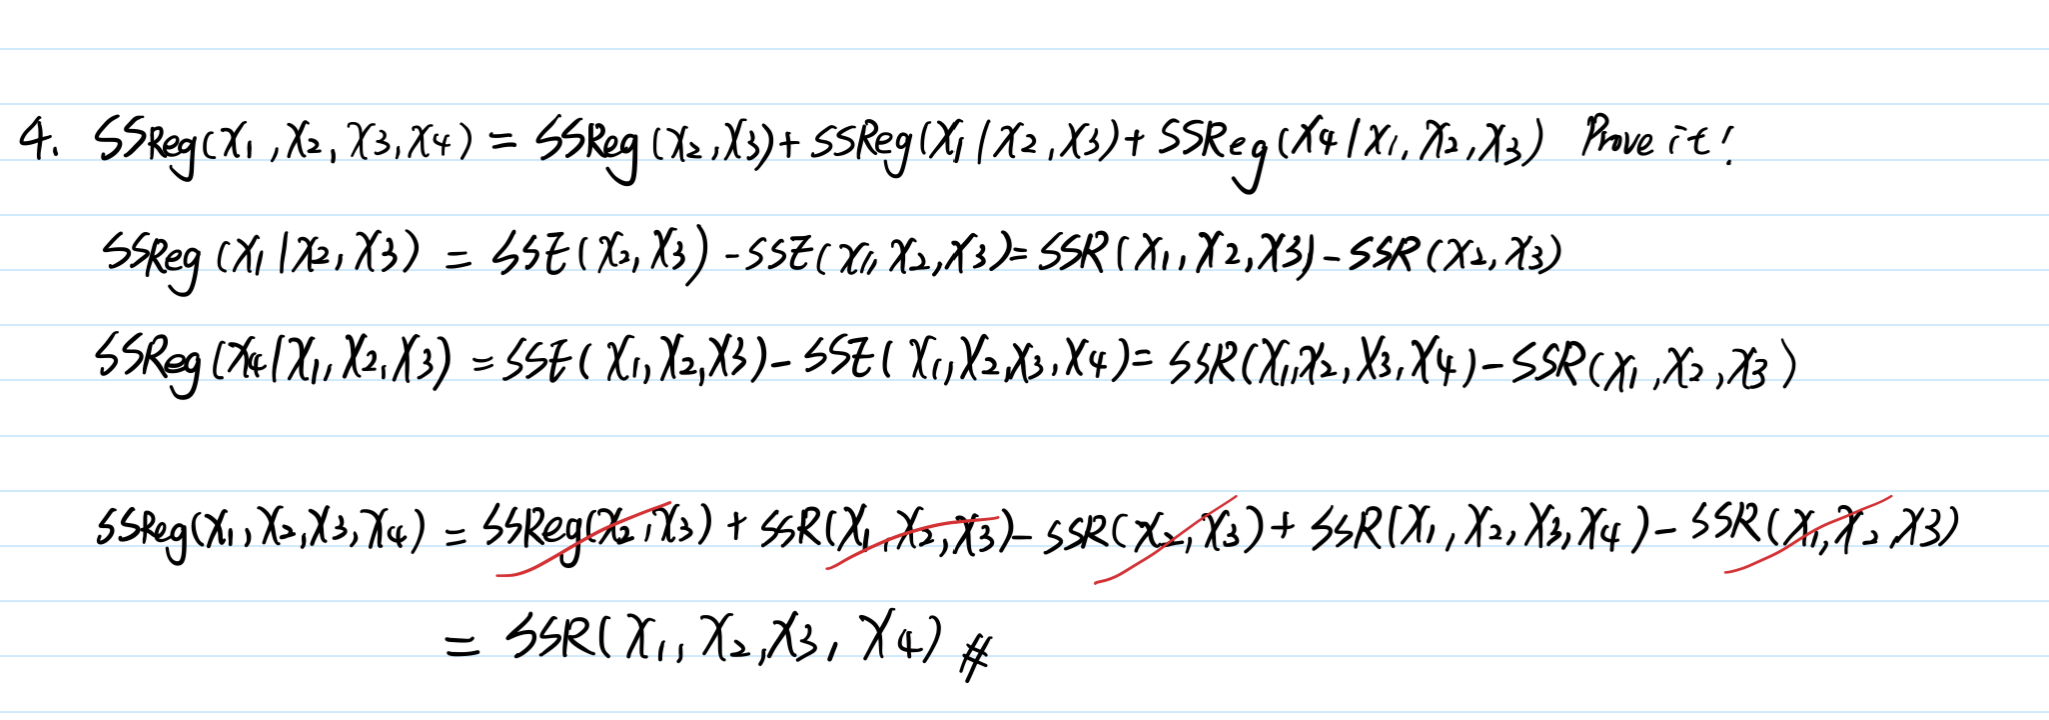
\includegraphics{pics/4.jpeg}

\begin{enumerate}
\def\labelenumi{\arabic{enumi}.}
\setcounter{enumi}{4}
\tightlist
\item
  (\textbf{7.3, 7.24, 7.30}) Continue working with the Brand Preference
  data, which are available on our Blackboard, on
  \url{http://statweb.lsu.edu/EXSTWeb/StatLab/DataSets/NKNWData/CH06PR05.txt},
  and in the previous homework.
\end{enumerate}

Recall the variables: It was collected to study the relation between
degree of brand liking (Y) and moisture content (X1) and sweetness (X2)
of the product.

\begin{enumerate}
\def\labelenumi{(\alph{enumi})}
\tightlist
\item
  Obtain the ANOVA table that decomposes the regression sum of squares
  into extra sum of squares associated \emph{with X1} and \emph{with X2,
  given X1}.
\end{enumerate}

\begin{Shaded}
\begin{Highlighting}[]
\NormalTok{brand <-}\StringTok{ }\KeywordTok{read.table}\NormalTok{(}\StringTok{"./data/CH06PR05.txt"}\NormalTok{)}
\NormalTok{brand }\OperatorTok
\StringTok{  }\KeywordTok{rename}\NormalTok{(}\DataTypeTok{Y =}\NormalTok{ V1, }\DataTypeTok{X1 =}\NormalTok{ V2, }\DataTypeTok{X2 =}\NormalTok{ V3) ->}\StringTok{ }\NormalTok{brand}

\CommentTok{# SSR(X1) }
\NormalTok{X1 <-}\StringTok{ }\KeywordTok{lm}\NormalTok{(Y }\OperatorTok{~}\StringTok{ }\NormalTok{X1, }\DataTypeTok{data =}\NormalTok{ brand)}

\CommentTok{# SSR(X2|X1)}
\NormalTok{X2givenX1 <-}\StringTok{ }\KeywordTok{lm}\NormalTok{(Y }\OperatorTok{~}\StringTok{ }\NormalTok{X1 }\OperatorTok{+}\StringTok{ }\NormalTok{X2, }\DataTypeTok{data =}\NormalTok{ brand)}

\KeywordTok{anova}\NormalTok{(X1)}
\end{Highlighting}
\end{Shaded}

\begin{verbatim}
## Analysis of Variance Table
## 
## Response: Y
##           Df  Sum Sq Mean Sq F value    Pr(>F)    
## X1         1 1566.45 1566.45  54.751 3.356e-06 ***
## Residuals 14  400.55   28.61                      
## ---
## Signif. codes:  0 '***' 0.001 '**' 0.01 '*' 0.05 '.' 0.1 ' ' 1
\end{verbatim}

\begin{Shaded}
\begin{Highlighting}[]
\KeywordTok{anova}\NormalTok{(X2givenX1)}
\end{Highlighting}
\end{Shaded}

\begin{verbatim}
## Analysis of Variance Table
## 
## Response: Y
##           Df  Sum Sq Mean Sq F value    Pr(>F)    
## X1         1 1566.45 1566.45 215.947 1.778e-09 ***
## X2         1  306.25  306.25  42.219 2.011e-05 ***
## Residuals 13   94.30    7.25                      
## ---
## Signif. codes:  0 '***' 0.001 '**' 0.01 '*' 0.05 '.' 0.1 ' ' 1
\end{verbatim}

\begin{enumerate}
\def\labelenumi{(\alph{enumi})}
\setcounter{enumi}{1}
\tightlist
\item
  Test whether X2 can be dropped from the model while X1 is retained.
\end{enumerate}

Consider dropping X2, the hypothesis is H0: \(\beta2 = 0\) = 0 vs
\(\beta2 \neq 0\). According to the analysis of variance table above,
the p-value of X2 is 2.011e-05, indicating that there is evidence that
\(beta2 neq 0\), so X2 cannot be removed from the model.

\begin{enumerate}
\def\labelenumi{(\alph{enumi})}
\setcounter{enumi}{2}
\tightlist
\item
  Fit first-order simple linear regression for relating brand liking (Y)
  to moisture content (X1).
\end{enumerate}

\begin{Shaded}
\begin{Highlighting}[]
\KeywordTok{summary}\NormalTok{(X1)}\OperatorTok{$}\NormalTok{coefficients[, }\DecValTok{1}\NormalTok{]}
\end{Highlighting}
\end{Shaded}

\begin{verbatim}
## (Intercept)          X1 
##      50.775       4.425
\end{verbatim}

\[
\hat{Y} = 50.775 + 4.425X1
\]

\begin{enumerate}
\def\labelenumi{(\alph{enumi})}
\setcounter{enumi}{3}
\tightlist
\item
  Compare the estimated regression coefficient for X1 with the
  corresponding coefficient obtained in (a).
\end{enumerate}

\begin{itemize}
\tightlist
\item
  In the \texttt{X2givenX1} model, the estimated regression coefficient
  for X1 is 4.425.
\item
  In the \texttt{X1} model, the estimated regression coefficient for X1
  is 4.425, too.
\end{itemize}

\begin{Shaded}
\begin{Highlighting}[]
\KeywordTok{summary}\NormalTok{(X2givenX1)}\OperatorTok{$}\NormalTok{coefficients[}\DecValTok{2}\NormalTok{,}\DecValTok{1}\NormalTok{]}
\end{Highlighting}
\end{Shaded}

\begin{verbatim}
## [1] 4.425
\end{verbatim}

\begin{Shaded}
\begin{Highlighting}[]
\KeywordTok{summary}\NormalTok{(X1)}\OperatorTok{$}\NormalTok{coefficients[}\DecValTok{2}\NormalTok{,}\DecValTok{1}\NormalTok{]}
\end{Highlighting}
\end{Shaded}

\begin{verbatim}
## [1] 4.425
\end{verbatim}

\begin{enumerate}
\def\labelenumi{(\alph{enumi})}
\setcounter{enumi}{4}
\tightlist
\item
  Does SSreg(X1) equal SSreg(X1\textbar X2) here? Is the difference
  substantial?
\end{enumerate}

\begin{itemize}
\tightlist
\item
  There are no different between sum of squares of X1. The first model
  SSReg(X1) is 1566.45, and the second model SSReg(X1\textbar X2) is
  1566.45.
\end{itemize}

\begin{Shaded}
\begin{Highlighting}[]
\CommentTok{# SSReg(X1)}
\KeywordTok{anova}\NormalTok{(X1)}
\end{Highlighting}
\end{Shaded}

\begin{verbatim}
## Analysis of Variance Table
## 
## Response: Y
##           Df  Sum Sq Mean Sq F value    Pr(>F)    
## X1         1 1566.45 1566.45  54.751 3.356e-06 ***
## Residuals 14  400.55   28.61                      
## ---
## Signif. codes:  0 '***' 0.001 '**' 0.01 '*' 0.05 '.' 0.1 ' ' 1
\end{verbatim}

\begin{Shaded}
\begin{Highlighting}[]
\CommentTok{# SSReg(X1|X2)}
\NormalTok{X1givenX2 <-}\StringTok{ }\KeywordTok{lm}\NormalTok{(Y }\OperatorTok{~}\StringTok{ }\NormalTok{X2 }\OperatorTok{+}\StringTok{ }\NormalTok{X1, }\DataTypeTok{data =}\NormalTok{ brand)}
\KeywordTok{anova}\NormalTok{(X1givenX2)}
\end{Highlighting}
\end{Shaded}

\begin{verbatim}
## Analysis of Variance Table
## 
## Response: Y
##           Df  Sum Sq Mean Sq F value    Pr(>F)    
## X2         1  306.25  306.25  42.219 2.011e-05 ***
## X1         1 1566.45 1566.45 215.947 1.778e-09 ***
## Residuals 13   94.30    7.25                      
## ---
## Signif. codes:  0 '***' 0.001 '**' 0.01 '*' 0.05 '.' 0.1 ' ' 1
\end{verbatim}

\begin{enumerate}
\def\labelenumi{(\alph{enumi})}
\setcounter{enumi}{5}
\item
\end{enumerate}

\begin{itemize}
\tightlist
\item
  Regress Y on X2 and obtain the residuals.
\end{itemize}

\begin{Shaded}
\begin{Highlighting}[]
\KeywordTok{residuals}\NormalTok{(}\KeywordTok{lm}\NormalTok{(Y }\OperatorTok{~}\StringTok{ }\NormalTok{X2 , }\DataTypeTok{data =}\NormalTok{ brand))}
\end{Highlighting}
\end{Shaded}

\begin{verbatim}
##       1       2       3       4       5       6       7       8       9      10 
## -13.375 -13.125 -16.375 -10.125  -5.375  -6.125  -6.375  -3.125   5.625   2.875 
##      11      12      13      14      15      16 
##   8.625   6.875  10.625   8.875  16.625  13.875
\end{verbatim}

\begin{itemize}
\tightlist
\item
  Regress X1 on X2 and obtain the residuals.
\item
  Regress residuals from the model ``Y on X2'' on residuals from the
  model ``X1 on X2''; compare the estimated slope, error sum of squares
  with \#1. What about \(R^2\)?
\end{itemize}

\begin{enumerate}
\def\labelenumi{\arabic{enumi}.}
\setcounter{enumi}{5}
\tightlist
\item
  (\textbf{8.13}) Consider a regression model Y = \(\beta0\) +
  \(\beta1\)X1 + \(\beta2\)X2 + e, where X1 is a numerical variable, and
  X2 is a dummy variable. Sketch the response curves (the graphs of E(Y)
  as a function of X1 for different values of X2), if \(\beta0\) = 25,
  \(\beta1\) = 0.2, and \(\beta2\) = −12.
\end{enumerate}

\begin{itemize}
\tightlist
\item
  The blue line indicates the association between E(Y) and X1 when X2 =
  0
\item
  The green line indicates the association between E(Y) and X1 when X2 =
  1
\end{itemize}

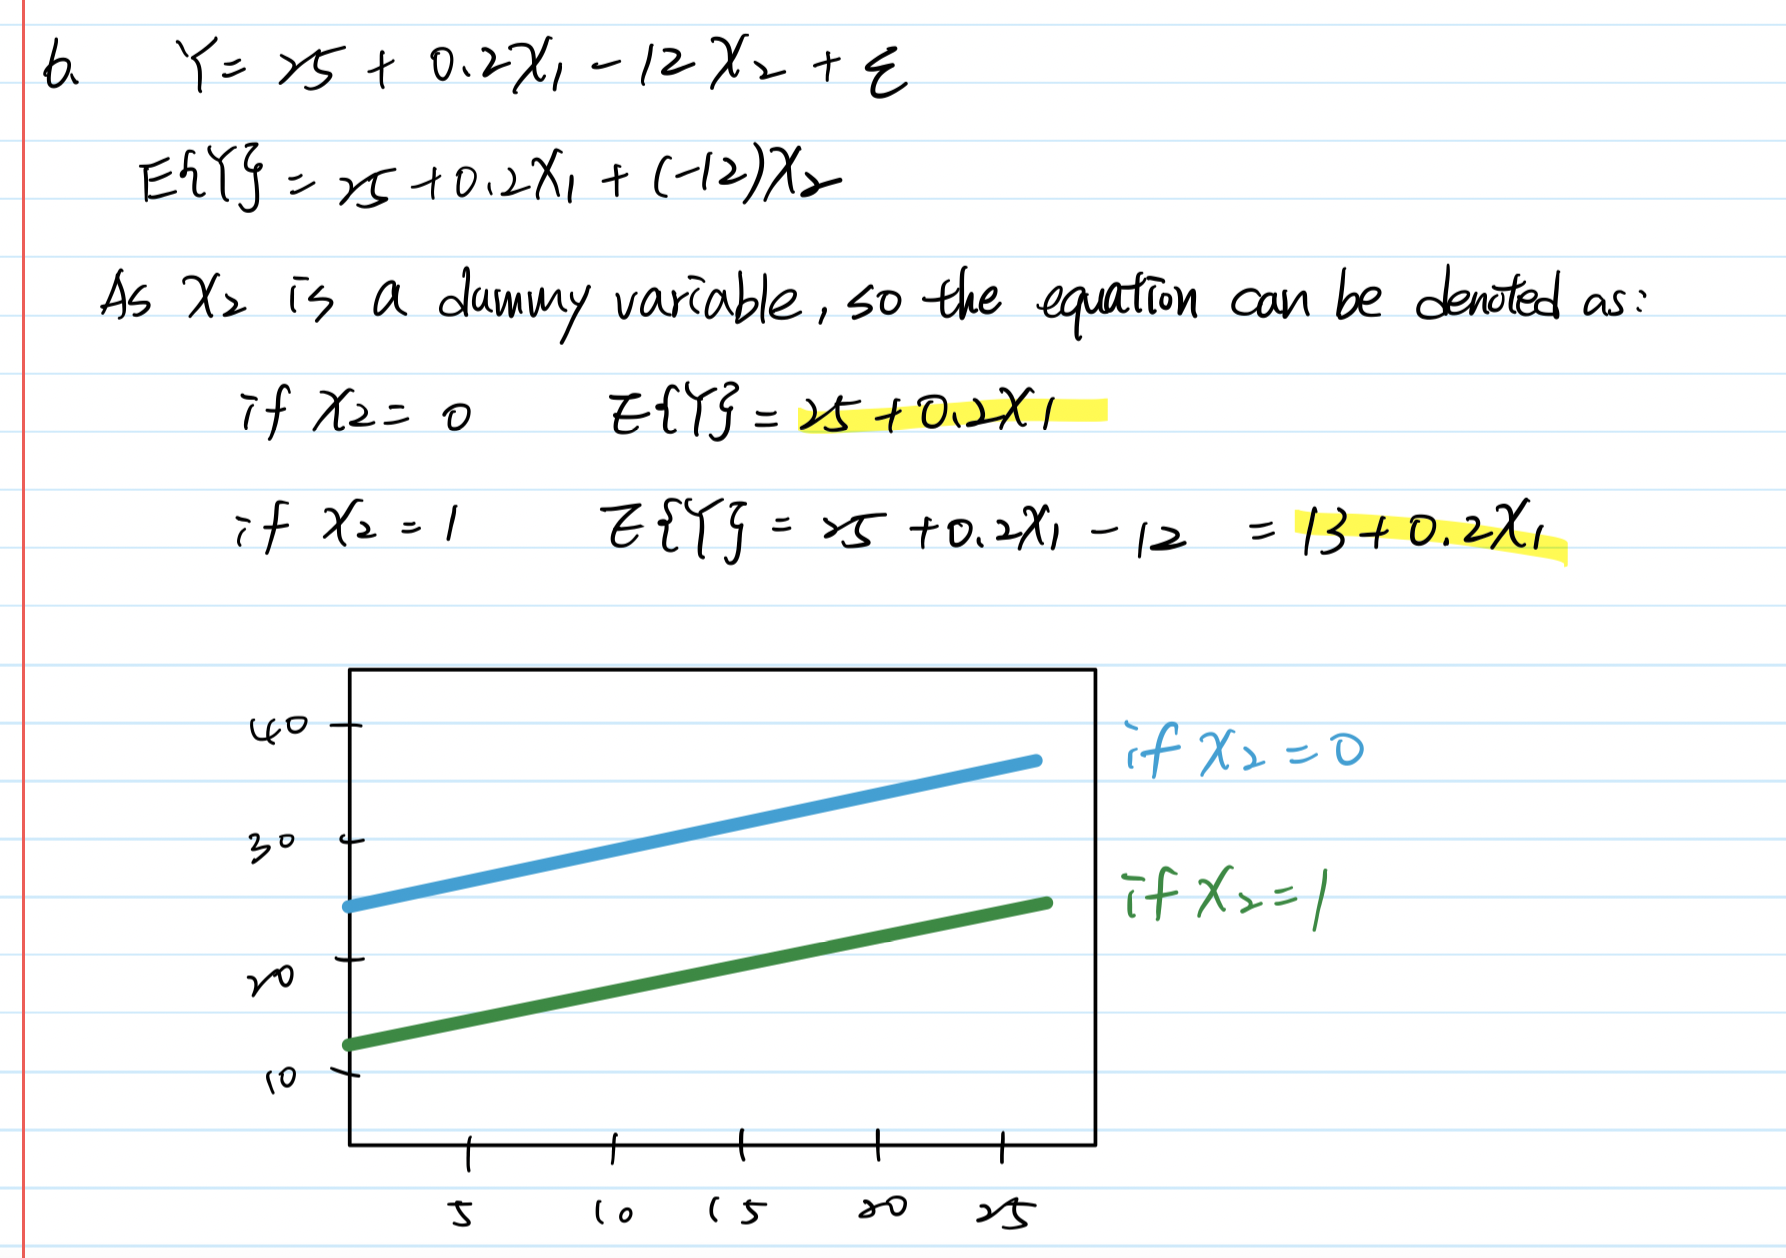
\includegraphics{pics/6.png}

\begin{enumerate}
\def\labelenumi{\arabic{enumi}.}
\setcounter{enumi}{6}
\tightlist
\item
  Continue the previous exercise. Sketch the response curves for the
  model with interaction, Y = \(\beta0\) + \(\beta1\)X1 + \(\beta2\)X2 +
  \(\beta3\)X1X2 + e, given that \(\beta3\) = −0.2
\end{enumerate}

\begin{itemize}
\tightlist
\item
  The red line indicates the association between E(Y) and X1 when X2 = 0
\item
  The green line indicates the association between E(Y) and X1 when X2 =
  1
\end{itemize}

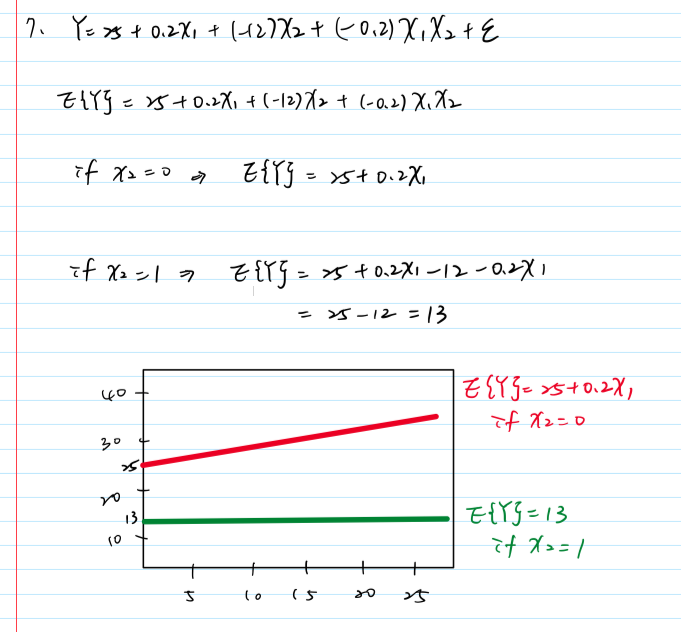
\includegraphics{pics/7.png}

\begin{enumerate}
\def\labelenumi{\arabic{enumi}.}
\setcounter{enumi}{7}
\tightlist
\item
  (\textbf{8.34}) In a regression study, three types of banks were
  involved, namely, (1) commercial, (2) mutual savings, and (3) savings
  and loan. Consider the following dummy variables for the type of bank:
\end{enumerate}

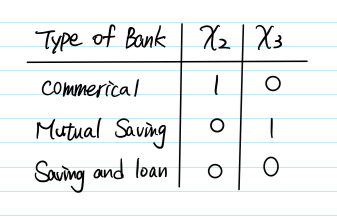
\includegraphics{pics/8.png}

\end{document}
